\boxde
\BTTN
\begin{ex}
    \immini{Cho hàm số $y=f(x)$ có bảng biến thiên như hình vẽ bên. Giá trị lớn nhất của hàm số đã cho trên tập hợp $\mathbb{R}$ bằng
        \choice
        {$-1$}
        {$1$}
        {$\dfrac{1}{3}$}
        {\True $3$}}{
        
\begin{tikzpicture}
            \tkzTabInit[nocadre=false,lgt=1.2,espcl=2,deltacl=0.6]
            {$x$ /0.6,$f’(x)$ /0.6,$f(x)$ /2}
            {$-\infty$, $-1$,$1$,$+\infty$}
            \tkzTabLine{,+,0,-,0,+,}
            \tkzTabVar{-/$1$,+/$3$,-/$\dfrac{1}{3}$,+/$1$}
    \end{tikzpicture}}
    \loigiai{
        Từ bảng biến thiên của hàm số $y=f(x)$ ta có $\max\limits_{\mathbb{R}}f(x)=3$ đạt được khi $x=-1$.
    }
\end{ex}

\begin{ex}%[2D1N3-1]
    \immini{Cho hàm số $y=f(x)$ liên tục trên $[-3 ; 2]$ và có bảng biến thiên như hình dưới đây. Gọi $M$ và $m$ lần lượt là giá trị lớn nhất và giá trị nhỏ nhất của hàm số $y=f(x)$ trên $[-1 ; 2]$. Giá trị của $5M-2m$ bằng bao nhiêu?
        \choice
        {\True $15$}
        {$3$}
        {$17$}
        {$-15$}}{
        
\begin{tikzpicture}
            \tkzTabInit[nocadre=false,lgt=1.1,espcl=1.6,deltacl=0.5]
            {$x$ /0.7,$y'$ /0.7,$y$ /2}
            {$-3$,$-1$,$0$,$1$,$2$}
            \tkzTabLine{,+,$0$,-,$0$,+,$0$,-,}
            \tkzTabVar{-/$2$,+/$3$,-/$0$,+/$2$,-/$1$}
    \end{tikzpicture}}
    \loigiai{
        Ta có $M=\max \limits_{[-1 ; 2]} f(x)=f(-1)=3$ và $m=\min\limits _{[-1 ; 2]} f(x)=f(0)=0$.\\
        Vậy $5M-2m=15$.
    }
\end{ex}

\begin{ex}%[2D1N3-1]
    \immini{Cho hàm số $y=f(x)$ có đồ thị như hình vẽ. Gọi $m$ và $M$ lần lượt là giá trị nhỏ nhất và giá trị lớn nhất của hàm số $f(x)$ trên đoạn $[-1 ; 1]$. Khẳng định nào sau đây là đúng?
        \choice
        {$m+M=2$}
        {$m+M=-2$}
        {$m+M=0$}
        {\True $m+M=-3$}}{
        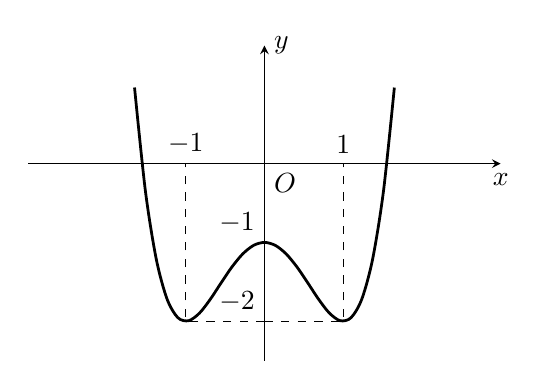
\begin{tikzpicture}[>=stealth]
            \draw[->] (-3,0) --(0,0) node[below
            right]{$O$} -- (3,0)
            node[below]{$x$};
            \draw[->](0,-2.5)--(0,1.5)
            node[right]{$y$};
            \draw[smooth,line width=1]
            plot[domain=-1.65:1.65]
            (\x,{(\x)^(4)-2*(\x)^(2)-1});
            \draw[dashed] (0,-2)
            node[left]{} -- (1,-2) --
            (1,0) node[above]{$1$};
            \draw[dashed] (0,-2)
            node[above left]{$-2$} -- (-1,-2) --
            (-1,0) node[above]{$-1$};
            \draw (0,-1) node[above left] {$-1$};
    \end{tikzpicture}}
    \loigiai{
        Dựa vào đồ thị, ta thấy trên đoạn $[-1 ; 1]$, hàm số đạt:\\
        Giá trị lớn nhất $M=-1$ tại $x=0$.\\
        Giá trị nhỏ nhất $m=-2$ tại $x= \pm1$.\\
        Suy ra $m+M=-3$.}
\end{ex}

\begin{ex}
    Hàm số $y=-\dfrac{1}{2}x^2+1013x+2024$ đạt giá trị lớn nhất tại điểm
    \choice
    { $x=2023$}
    {\True $x=2026$}
    {$x=2024$ }
    {$x=1013$ }
    \loigiai{
        Tập xác định $\mathbb{R}$.\\
        $y'=-\dfrac{1}{2}x+1013$, \quad $y'=0 \Leftrightarrow -\dfrac{1}{2}x+1013=0 \Leftrightarrow x=2026$.\\
        Bảng biến thiên:
        \begin{center}
            
\begin{tikzpicture}
                \tkzTabInit[nocadre=false,lgt=1,espcl=2.5]
                {$x$ /0.6,$y'$ /0.6,$y$ /2}
                {$-\infty$,$0$,$+\infty$}
                \tkzTabLine{,+,$2026$,-,}
                \tkzTabVar{-/$-\infty$, +/,-/$-\infty$}
            \end{tikzpicture}
        \end{center}
        Suy ra, hàm số đạt giá trị lớn nhất tại điểm $x=2026$.
    }
\end{ex}

\begin{ex}
    Trên đoạn $[-1;2]$, hàm số $y=x^3+3x^2+1$ đạt giá trị nhỏ nhất tại điểm
    \choice
    {$x=2$}
    {\True $x=0$}
    {$x=-1$}
    {$x=1$}
    \loigiai{Hàm số $y=x^3+3x^2+1$ liên tục trên đoạn $[-1;2]$.\\
        Ta có $y'=3x^2+6x$.\\
        Cho $y'=0\Leftrightarrow \hoac{&x=0\in [-1;2]\\&x=-2\notin [-1;2].} $
        \begin{itemize}
            \item Khi $x=0\Rightarrow y=1$.
            \item Khi $x=-1\Rightarrow y=3$.
            \item Khi $x=2\Rightarrow y=13$.
        \end{itemize}
        Vậy trên đoạn $[-1;2]$ hàm số đạt giá trị nhỏ nhất tại điểm $x=0$.
    }
\end{ex}

\begin{ex}%[THPTQG 2020-2 - mã đề 102]%[Quảng Đại Mưa]%[2D1B3-1]
    Giá trị nhỏ nhất của hàm số $f(x)=x^{4}-12 x^{2}-4$ trên đoạn $\left[0 ; 9\right]$ bằng
    \choice
    {$-39$}
    {\True$-40$}
    {$-36$}
    { $-4$}
    \loigiai{
        $\bullet$ Ta có $f'(x)=4x^{3}-24 x ; f'(x)=0 \Leftrightarrow\hoac{
            &x=0 \\&
            x=\sqrt{6}\\&x=-\sqrt{6}~~ \text{(loại).}}$\\
        $\bullet$ Tính được $f(0)=-4 ; f(9)=5585$ và $f(\sqrt{6})=-40.$\\
        $\bullet$  Do đó $\min\limits_{\left[0;9\right]}f(x)=-40.$

    }
\end{ex}


\begin{ex}%[2D1N3-1]
    Giá trị nhỏ nhất của hàm số $f(x)=\dfrac{x^2+3}{x-1}$ trên đoạn $[2 ; 4]$ là
    \choice
    {$7$}
    {\True $6$}
    {$\dfrac{19}{3}$}
    {$\dfrac{13}{3}$}
    \loigiai{
        Xét hàm số $f(x)=\dfrac{x^2+3}{x-1}$ trên $[2 ; 4]$, có $f'(x)=\dfrac{x^2-2 x-3}{(x-1)^2}$\\
        Phương trình $f'(x)=0 \Leftrightarrow $ $\heva{&2 \leq x \leq 4 \\ & x^2-2x-3=0 }$
        $ \Leftrightarrow x=3.$\\
        Tính $f(2)=7 ; f(3)=6 ; f(4)=\dfrac{19}{3}  $.\\
        Vậy $\min\limits _{[2 ; 4]} f(x)=f(3)=6  $.
    }
\end{ex}

\begin{ex}%[2D1N3-1]
    Gọi $M$ và $m$ lần lượt là giá trị lớn nhất và giá trị nhỏ nhất của hàm số $y=\sqrt{1-x}+\sqrt{1+x}$. Giá trị của $M-2 m^2$ bằng
    \choice
    {\True $-2$}
    {$2$}
    {$0$}
    {$-1$}
    \loigiai{Điều kiện xác định $\heva{&1-x \geq 0  \\& x+1 \geq 0} \Leftrightarrow-1 \leq x \leq              1$.\\
        Xét hàm số $f(x)=\sqrt{1-x}+\sqrt{1+x}$ trên $[-1 ; 1]$, có $f'(x)=-\dfrac{1}{2 \sqrt{1-x}}+\dfrac{1}{2 \sqrt{1+x}}$;\\
        Phương trình $f'(x)=0 \Leftrightarrow \heva{&-1<x<1 \\& \sqrt{1-x}=\sqrt{1-x}} \Leftrightarrow x=0 $. \\
        Tính $f(-1)=f(1)=\sqrt{2} ; f(0)=2$.\\
        Vậy $\heva{&m=\min\limits _{[-1 ; 1]} f(x)=\sqrt{2} \\& M=\max \limits_{[-1 ; 1]} f(x)=2}\rightarrow M-2 m^2=2-2\cdot2=-2$.
    }
\end{ex}

\begin{ex}%[2D1N3-2]
    Giá trị lớn nhất của hàm số $y=-x^3+3 x+1$ trên khoảng $(0 ;+\infty)$ bằng
    \choice
    {$1$}
    {\True $3$}
    {$-1$}
    {$5$}
    \loigiai{Ta có $y'=-3 x^2+3$,  $y'=0         \Leftrightarrow \heva{&x=1\in(0 ;+\infty) \\&x=-1 \notin(0 ;+\infty)}$.\\
        Bảng biến thiên
        \begin{center}
            
\begin{tikzpicture}
                \tkzTabInit[nocadre=false,lgt=0.7,espcl=2.5,deltacl=0.5]
                {$x$ /0.7,$y'$ /0.7,$y$ /2}
                {$0$,$1$,$+\infty$}
                \tkzTabLine{,+,$0$,-,}
                \tkzTabVar{-/$1$,+/$3$,-/$-\infty$}
            \end{tikzpicture}
        \end{center}
        Từ bảng biến thiên ta thấy giá trị lớn nhất của hàm số $y=-x^3+3 x+1$ trên khoảng $(0 ;+\infty)$ bằng 3.}
\end{ex}

\begin{ex}%[2D1H3-1]
    Tìm giá trị thực của tham số $a$ để hàm số $f(x)=-x^3-3 x^2+a$ có giá trị nhỏ nhất trên đoạn $[-1 ; 1]$ bằng 0.
    \choice
    {$a=2$}
    {$a=6$}
    {$a=0$}
    {\True $a=4$}
    \loigiai{Xét hàm số $f(x)=-x^3-3 x^2+a$ trên $[-1 ; 1]$, có   $f'(x)=-3 x^2-6 x.$\\
        Phương trình $f'(x)=0 \Leftrightarrow \heva{&-1 \leq x \leq 1 \\& -3 x^2-6 x=0} \Rightarrow x=0$.\\
        Tính $f(-1)=-2+a ; f(0)=a ; f(1)=-4+a.$\\
        Suy ra $\min \limits_{[-1: 1]} f(x)=f(1)=-4+a=0 \Rightarrow a=4$.
    }
\end{ex}

\begin{ex}%[2D1H3-3]
    \immini{Cho hàm số $y=f(x)$ liên tục trên $\mathbb{R}$ và có đồ thị như hình bên. Tìm giá trị lớn nhất của hàm số $y=f^2(x)+3$ trên đoạn $[0 ; 2]$.
        \choice
        {\True $12$}
        {$13$}
        {$2$}
        {$9$}}{
        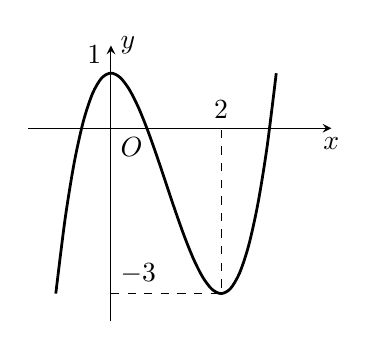
\begin{tikzpicture}[>=stealth,scale=0.7]
            \draw[->] (-1.5,0) --(0,0) node[below
            right]{$O$} -- (4,0)
            node[below]{$x$};
            \draw[->](0,-3.5)--(0,1.5)
            node[right]{$y$};
            \draw[smooth,line width=1]
            plot[domain=-1:3]
            (\x,{(\x)^(3)-3*(\x)^(2)+1});
            \draw[dashed] (0,-3) node[left]{} -- (2,-3) --
            (2,0) node[above]{$2$};
            \draw (0,-3) node[above right] {$-3$};
            \draw (0,1) node[above left] {$1$};
    \end{tikzpicture}}
    \loigiai{
        Đặt $g(x)=f^2(x)+3$. Từ đồ thị đã cho ta có $\exists x_0 \in(0 ; 1)$ để $f\left(x_0\right)=0$.
        $$
        \begin{gathered}
            \text { Và } \forall x \in[0 ; 2] \text { thì }-3 \leq f(x) \leq 1 \Rightarrow 0 \leq f^2(x) \leq 9 \Rightarrow 3 \leq f^2(x)+3 \leq 12 \Rightarrow 3 \leq g(x) \leq 12 \\
            \Rightarrow \max _{[0 ; 2]} g(x)=12 \text { khi } f(x)=-3 \Leftrightarrow x=2 \in[0 ; 2] .
        \end{gathered}
        $$}
\end{ex}


\begin{ex}%[2D1V3-1]
    Cho hàm số $f(x)$ có đạo hàm $f'(x)=(x+1)(x-1)^2(x-2)$. Giá trị nhỏ nhất của hàm số $g(x)=f(x)+\dfrac{1}{3} x^3-x-2$ trên đoạn $[-1 ; 2]$ bằng
    \choice
    {$f(2)-\dfrac{4}{3}$}
    {\True $f(1)-\dfrac{8}{3}$}
    {$f(0)-2$}
    {$f(-1)-\dfrac{4}{3}$}
    \loigiai{
        Ta có $g'(x)=f'(x)+x^2-1$.\\
        Khi đó $g'(x)=0 \Leftrightarrow(x+1)(x-1)^2(x-2)+x^2-1=0 \\
        \Leftrightarrow\left(x^2-1\right)\left(x^2-3 x+3\right)=0 \Leftrightarrow x= \pm 1$.\\
        Do phương trình $x^2-3 x+3=0$ vô nghiệm.\\
        Bảng biến thiên
        \begin{center}
            
\begin{tikzpicture}
                \tkzTabInit[nocadre=false,lgt=1.5,espcl=2.1,deltacl=0.7]
                {$x$ /0.7,$g'(x)$ /0.7,$g(x)$ /2}
                {$-1$,$1$,$2$}
                \tkzTabLine{,-,$0$,+,}
                \tkzTabVar{+/$ $,-/$g(1)$,+/$ $}
            \end{tikzpicture}
        \end{center}
        Hàm số đạt giá trị nhỏ nhất tại $x=1$ và GTNN bằng $g(1)=f(1)-\dfrac{8}{3}$.}
\end{ex}

\begin{ex}%[2D1V3-1]
    Cho hàm số $f(x)=\dfrac{x-m^2}{x+8}$ với $m$ là tham số thực. Tìm giá trị lớn nhất của $m$ để hàm số có giá trị nhỏ nhất trên đoạn $[0 ; 3]$ bằng $-2$.
    \choice
    {$m=-4$}
    {$m=5$}
    {\True $m=4$}
    {$m=1$}
    \loigiai{
        Xét hàm số $f(x)=\dfrac{x-m^2}{x+8}$ trên $[0 ; 3]$, có $f'(x)=\dfrac{8+m^2}{(x+8)^2}>0 , \forall x \in[0 ; 3]$\\
        Suy ra $f(x)$ là hàm số đồng biến trên $(0 ; 3) \Rightarrow \min \limits _{[0 ; 3]} f(x)=f(0)=-\dfrac{m^2}{8}$\\
        Theo bài ta, ta có $\min \limits _{[0 ; 3]} f(x)=-2 \Leftrightarrow-\dfrac{m^2}{8}=-2 \Leftrightarrow m^2=16 \Rightarrow m_{\max }=4$.
    }
\end{ex}

\begin{ex}
    Cho hàm số $ f(x)=mx^4+2(m-1)x^2 $ với $ m $ là tham số thực. Nếu $ \min\limits_{[0;2]} f(x)=f(1) $ thì $ \max\limits_{[0;2]} f(x) $ bằng
    \choice
    {$ 2 $}
    {$ -1 $}
    {\True $ 4 $}
    {$ 0 $}
    \loigiai{
        Ta có $ f'(x)=4mx^3+4(m-1)x $.
        \begin{itemize}
            \item Với $ m=0 $ thì $ f(x)=-2x^2 $ là hàm số nghịch biến trên $ (0;2) $.\\
            Khi đó $ \min\limits_{[0;2]} f(x)=f(2) $ (không thỏa yêu cầu bài toán).
            \item Với $ m\neq 0 $ thì hàm số $ y=f(x) $ có đồ thị nhận $ Oy $ làm trục đối xứng và luôn có một điểm cực trị $ x=0 $.\\
            Khi đó, từ yêu cầu bài toán ta suy ra $ \left\{\begin{aligned}
                & m>0\\
                & f'(1)=0
            \end{aligned}\right. \Leftrightarrow \left\{\begin{aligned}
                & m>0\\
                & 4m+4(m-1)=0
            \end{aligned}\right. \Leftrightarrow m=\dfrac{1}{2}\cdot $ \\
            Do đó $ f'(x)=2x^3-2x $; $ f'(x)=0 \Leftrightarrow \left[\begin{aligned}
                & x=-1\notin (0;2)\\
                & x=0\notin (0;2)\\
                & x=1\in (0;2).
            \end{aligned}\right. $ \\
            Ta có $ f(0)=0 $, $ f(2)=4 $, $ f(1)=-\dfrac{1}{2}\cdot $
        \end{itemize}
        Vậy $ \max\limits_{[0;2]} f(x)=4 $ tại $ x=2 $.
    }
\end{ex}

\begin{ex}%[2D1T3-6]
    Một trang trại mỗi ngày thu hoạch được một tấn rau. Mỗi ngày, nếu bán rau với giá $30000$ đồng/kg thì hết rau, nếu giá bán cứ tăng thêm $1000$ đồng/kg thì số rau thừa lại tăng thêm $20$ kg. Số rau thừa này được bán để làm thức ăn cho gia súc với giá $2000$ đồng/kg. Hỏi số tiền bán rau nhiều nhất mà trang trại có thể thu được mỗi ngày là bao nhiêu?
    \choice
    {\True $32 420 000$ đồng}
    {$32 400 000$ đồng}
    {$34 400 000$ đồng}
    {$32 240 000$ đồng}
    \loigiai{Gọi $x$ (kg) là số rau thừa lại  với $0 \le x \le 1000$. \\
        Theo đề bài, ta được $\dfrac{x}{20}$ là số lần giá bán tăng thêm. \\
        Do đó ta được số tiền bán rau với giá $30000+\dfrac{x}{20} \cdot 1000$ là $\left(30000 +1000 \cdot \dfrac{x}{20}\right)(1000-x)$ đồng.\\
        Số tiền bán $x$ (kg) rau thừa để làm thức ăn gia súc là $2000x$ đồng.\\
        Vậy số tiền bán rau trang trại thu được là \\ $\left(30000 +1000 \cdot \dfrac{x}{20}\right)(1000-x)+2000x=-50x^2+22000x+30 000 000$ đồng.\\
        Xét hàm số $f(x)=-50x^2+22000x+30 000 000$ trên $[0;1000]$.\\
        Ta có $f'(x)=-100x+22000$.\\
        \hspace*{1cm} $f'(x)=0 \Leftrightarrow x=220$.\\
        Vì $f(0)=3 000 000$, $f(220)=32420000$, $f(1000)=20000000$ nên giá trị lớn nhất của $f(x)$ trên $[0;1000]$ là $32420000$.\\
        Vậy số tiền bán rau nhiều nhất mà trang trại có thể thu được mỗi ngày là $32420000$ đồng.
    }
\end{ex}

\BTTF
\begin{ex}%[2D1N3-1]
    Cho hàm số $y=f(x)$ xác định trên tập  $\mathscr{D}$ và một số thực $M$. Xét tính đúng sai của các khẳng định sau:
    \choiceTF
    {Nếu $f(x) \leq M,\,\forall x \in \mathscr{D}$ thì $\max\limits_{\mathscr{D}}f(x)=M$}
    {Nếu $f(x) \geq M,\,\forall x \in \mathscr{D}$ thì $\min\limits_{\mathscr{D}}f(x)=M$}
    {\True Nếu $f(x) = M,\,\forall x \in \mathscr{D}$ thì $\max\limits_{\mathscr{D}}f(x)=M$}
    {\True Nếu $f(x) = M ,\,\forall x \in \mathscr{D}$ thì $\min\limits_{\mathscr{D}}f(x)=M$}
    \loigiai{
        \begin{itemchoice}
            \itemch Khẳng định này sai, cần bổ sung thêm điều kiện $\exists x_0 \in \mathscr{D}$ để $f(x_0)=M$.
            \itemch Khẳng định này sai, cần bổ sung thêm điều kiện $\exists x_0 \in \mathscr{D}$ để $f(x_0)=M$.
            \itemch Nếu $f(x) = M,\,\forall x \in \mathscr{D}$ thì  $f(x)$ là hàm hằng trên $\mathscr{D}$ (đồ thị là đường thẳng nằm ngang). Suy ra $\max\limits_{\mathscr{D}}f(x)=M$.
            \itemch Nếu $f(x) = M,\,\forall x \in \mathscr{D}$ thì  $f(x)$ là hàm hằng trên $\mathscr{D}$ (đồ thị là đường thẳng nằm ngang). Suy ra $\min\limits_{\mathscr{D}}f(x)=M$.
        \end{itemchoice}
    }
\end{ex}

\begin{ex}
    \immini{Cho hàm số $y=f(x)$ xác định, liên tục trên $\mathbb{R}$ và có bảng biến thiên như hình bên. Xét tính đúng sai của các khẳng định sau:
        \choiceTF
        {Hàm số đồng biến trên khoảng $(-2;5)$}
        {\True Hàm số đạt cực đại tại điểm $x=-2$}
        {Hàm số có giá trị nhỏ nhất bằng $-2$}
        {\True Hàm số có giá trị lớn nhất bằng $5$}}{
        
\begin{tikzpicture}
            \tkzTabInit[nocadre=false,lgt=1.2,espcl=2.1,deltacl=0.6]
            {$x$ /0.7, $f’(x)$ /0.7, $f(x)$ /2.6}
            {$-\infty$,$-3$,$-2$,$+\infty$}
            \tkzTabLine{ ,+,$0$,+,$0$,-, }
            \tkzTabVar{-/$-2$,R,+/$5$,-/$-2$}
            \tkzTabIma{1}{3}{2}{$0$}
    \end{tikzpicture}}
    \loigiai{
        Hàm só $y=f(x)$ không có giá trị nhỏ nhất nên phát biểu ``Hàm số $y=f(x)$ có giá trị nhỏ nhất bằng $-\infty$'' là phát biểu sai.
    }
\end{ex}

\begin{ex}
    Cho hàm số $y = x^2 - 4\ln (1 - x)$. Xét tính đúng sai của các khẳng định sau:
    \choiceTF
    {Tập xác định của hàm số là $\mathscr{D}=(1;+\infty)$}
    {\True Đạo hàm của hàm số là $y'=\dfrac{-2x^2 + 2x + 4}{1 - x}$}
    {Giá trị lớn nhất của hàm số trên $[-2;0]$ là $2$}
    {\True Giá trị nhỏ nhất của hàm số trên $[-2;0]$ là $1 -4\ln 2$}
    \loigiai{
        Tập xác định: $\mathscr{D} = (-\infty;1)$.\\
        Ta có $y' = 2x + \dfrac{4}{1 - x} = \dfrac{-2x^2 + 2x + 4}{1 - x}$.\\
        Khi đó $y' = 0 \Leftrightarrow -2x^2 + 2x + 4 = 0 \Leftrightarrow \hoac{&x = -1 \quad \mbox{(nhận)} \\&x = 2 \quad \mbox{(loại)}. }$\\
        Khi đó $\heva{& y(-2) = 4 - 4\ln 3 \approx -0{,}4 \\& y(-1) = 1 - 4\ln 2  \approx -1{,}7\\& y(0) = 0.} \Rightarrow M = 0, N = 1 -4\ln 2$\\
        Vậy $M - N = 4\ln 2 -1$.
    }
\end{ex}

\begin{ex}%[2D1V3-6]
    \immini{Người ta muốn xây một bể bơi có dạng hình hộp chữ nhật, thể tích $1\,800$ m$^3$ và chiều sâu $2$ m (hình bên). Biết rằng chi phí xây mỗi đơn vị diện tích của đáy bể gấp hai lần so với thành bể. Gọi $x$ (m) và $y$ (m) là hai kích thước của mặt đáy.}
    {\begin{tikzpicture}[>=stealth,line join=round,line cap=round,font=\footnotesize,scale=0.65]
            \path
            (0,0) coordinate (A)
            (-1.3,-2) coordinate (B)
            (5,0) coordinate (D)
            ($(B)+(D)-(A)$) coordinate (C)
            ($(A)+(0,0.7)$) coordinate (A')
            ($(A')+(B)-(A)$) coordinate (B')
            ($(A')+(C)-(A)$) coordinate (C')
            ($(A')+(D)-(A)$) coordinate (D')


            ;
            \draw (B')--(A')--(D')--(C')--(B')--(B)--(C)--(C')(D')--(D)--(C) ;
            \draw[dashed](B)--(A)--(A')(D)--(A);
            \draw (B)--(C)node[pos=0.5,below]{$x$};
            \draw (C)--(D)node[pos=0.5,right]{$y$};
            \draw (D')--(D)node[pos=0.5,right]{$2$};
    \end{tikzpicture}}
    \choiceTF
    {Thể tích bể bơi được tính theo công thức $V=2x^2y$}
    {\True Mối liên hệ giữa $x$ và $y$ là $y=\dfrac{900}{x}$}
    {Tổng diện tích mặt bên của bể tính theo $x$, $y$ là $S=4(x+y)$}
    {\True  Để tổng chi phí xây dựng (bao gồm mặt đáy và mặt bên) nhỏ nhất thì cần chọn chiều dài là 40 m}
    \loigiai{
        \begin{itemchoice}
            \itemch Thể tích của bể là $V=B\cdot h=xy \cdot h$.
            \itemch Với $V=xy \cdot h \Rightarrow 1800 = xy \cdot 2 \Rightarrow xy=\dfrac{1800}{2}=900$.
            \itemch Tổng diện tích mặt bên gồm 4 hình chữ nhật (trước, sau, trái, phải) là
            $$S=2x+2x+2y+2y=4x+4y=4(x+y).$$
            \itemch Tổng diện tích của bể là $4x+4y+xy=4x+4\cdot \dfrac{900}{x}+900$.\\
            Vì chi phí xây mỗi đơn vị diện tích của đáy bể gấp hai lần so với thành bể nên chi phí cần có là $4x+4\cdot \dfrac{900}{x}+2\cdot 900$.\\
            Đặt $f(x)=4x+4\cdot \dfrac{900}{x}+1\,800$.\\
            $f'(x)=4-\dfrac{3\,600}{x^2}$;\quad
            $f'(x)=0\Leftrightarrow x=30$ (do $x>0$).\\
            Bảng biến thiên
            \begin{center}
                
\begin{tikzpicture}
                    \tkzTabInit[nocadre=false, lgt=1.2, espcl=2.4]{$x$ /0.7,$f'(x)$ /0.7,$f(x)$ /2}{$0$,$30$,$+\infty$}
                    \tkzTabLine{,-,$0$,+,}
                    \tkzTabVar{+/  ,-/$2\,040$,+/$+\infty$}
                \end{tikzpicture}
            \end{center}
            Với $x=30$m vaf $y=30$ m và thì chi phí xây dựng bể là thấp nhất.
        \end{itemchoice}
    }
\end{ex}

\BTTL

\begin{ex}%[Nguồn]%[Toanvo, dự án]%[2D1B3-1]
    Giá trị nhỏ nhất của hàm số $f(x)=x^3-30x$ trên đoạn $\left[2;19\right]$ bằng bao nhiêu? (làm tròn đến hàng phần chục)\\
    \shortans[3]{$-63{,}2$}
    \loigiai{
        Hàm số đã cho xác định và liên tục trên đoạn $\left[2;19\right]$.\\
        Ta có $f'\left(x\right)=3x^2-30;f'\left(x\right)=0\Leftrightarrow\left[\begin{array}{l}
            x=\sqrt{10}\in\left[2;19\right]\\
            x=-\sqrt{10}\notin\left[2;19\right].
        \end{array}\right.$\\
        Mà $f\left(2\right)=-52;f\left(\sqrt{10}\right)=-20\sqrt{10}\approx-63,25;f\left(19\right)=6289$.\\
        Vậy $\min\limits_{\left[2;19\right]}f\left(x\right)=-20\sqrt{10} \approx -63{,}2$.
    }
\end{ex}

\begin{ex}%[2017CT-104] %[2D1T3]
    Một vật chuyển động theo quy luật $s=-\dfrac{1}{3} t^3 + 6 t^2$ với $t$ (giây) là khoảng thời gian tính từ khi vật bắt đầu chuyển động và $s$ (mét) là quãng đường vật di chuyển được trong khoảng thời gian đó. Hỏi trong khoảng thời gian 9 giây, kể từ khi bắt đầu chuyển động, vận tốc (m/s) lớn nhất của vật đạt được bằng bao nhiêu?\\
    \shortans[3]{$36$}
    \loigiai{
        Vận tốc của vật được tính bởi: $v(t)=-t^2+12t$.
        Ta có $v'(t)=-2t+12$.
        Bảng biến thiên:
        \begin{center}
            
\begin{tikzpicture}
                \tkzTabInit[nocadre,lgt=1,espcl=3]
                {$t$ /0.6, $v'$ /.6,$v$ /1.8}
                {$0$ ,$6$ ,$9$}
                \tkzTabLine{,+,0,-,}
                \tkzTabVar{ -/$0$,+/$36$,-/$27$}
            \end{tikzpicture}
        \end{center}
        Dựa vào bảng biến thiên ta có vận tốc lớn nhất của vật đạt được bằng $36$ m/s.
    }
\end{ex}

\begin{ex}%[2D1H3-1]
    Gọi $m$ và $M$ lần lượt là giá trị nhỏ nhất và giá trị lớn nhất của hàm số $y=\dfrac{1}{2} x-\sqrt{x+2}$ trên đoạn $[-1 ; 34]$. Tổng $S=3m+M$ bằng bao nhiêu?\\
    \shortans[3]{$6,5$}
    \loigiai{
        Ta có $y'=\dfrac{1}{2}-\dfrac{1}{2\sqrt{x+2}}=\dfrac{\sqrt{x+2}-1}{2 \sqrt{x+2}}$.\\
        $y'=0 \Leftrightarrow \sqrt{x+2}=1 \Leftrightarrow x=-1 \in [-1 ; 34]$\\
        $f(-1)=-\dfrac{3}{2} ; f(34)=11 $\\
        Vậy $m=-\dfrac{3}{2} ; M=11 \Rightarrow S=3\left(-\dfrac{3}{2}\right)+11=\dfrac{-9}{2}+11=\dfrac{13}{2}=6{,}5$.
    }
\end{ex}
\begin{ex} %[2D1V3-1]
    Cho hàm số $y=(x+m)^3-3(x+m)+1+n$. Biết hàm số nghịch biến trên khoảng $(0 ; 2)$ và giá trị lớn nhất của hàm số trên $[-1 ; 1]$ bằng 4. Tính $m+n$.
    \shortans[3]{$0$}
    \loigiai{
        $$\begin{aligned}
            & y'=3(x+m)^2-3=3(x+m+1)(x+m-1) \\
            & y'=0 \Leftrightarrow \hoac{&x=1-m=x_2 \\ &x=-1-m=x_1.}
        \end{aligned}$$
        Để hàm số nghịch biến trên $(0 ; 2)$ thì \\
        $\heva{
            &3 \cdot y ^ { \prime } ( 0 ) \leq 0 \\
            &3 \cdot y ^ { \prime } ( 2 ) \leq 0 }
        \Leftrightarrow
        \heva{
            & y ^ { \prime } ( 0 ) \leq 0  \\
            & y ^ { \prime } ( 2 ) \leq 0 }
        \Leftrightarrow
        \heva{
            &3 m ^ { 2 } - 3 \leq 0  \\
            & 3 ( 2 + m ) ^ { 2 } - 3 \leq 0 }
        \Leftrightarrow
        \heva{
            & m^2-1 \leq 0 \\
            & (2+m)^2-1 \leq 0}\\
        \Leftrightarrow
        \heva{
            & - 1 \leq m \leq 1  \\
            & - 1 \leq 2 + m \leq 1 }
        \Leftrightarrow
        \heva{
            & -1 \leq m \leq 1 \\
            & -3 \leq m \leq-1}
        \Leftrightarrow
        m=-1.$\\
        Với $m=-1$ thì $y'=0 \Leftrightarrow \hoac{&x=0 \in[-1 ; 1] \\ &x=2 \notin[-1 ; 1].}$\\
        Ta có $y(0)=n+3, y(1)=n+1, y(-1)=n-1 \Rightarrow \max \limits _{[-1 ; 1]} y=n+3=4 \Rightarrow n=1.$\\
        $\Rightarrow m+n=0$.
    }
\end{ex}

\begin{ex}%[2D1C3-6]
    Một cửa hàng bán vải Thanh Hà với giá bán mỗi kg là $50\,000$ đồng. Với giá bán này thì cửa hàng chi bán được khoảng $25$ kg. Cửa hàng này dự định giảm giá bán, ước tính nếu cửa hàng cứ giảm $4000$ đồng cho một kg thì số vải bán được tăng thêm là $50 \mathrm{~kg}$. Xác định giá bán (đơn vị nghìn đồng) đề cửa hàng đó thu được lợi nhuận lớn nhất, biết rằng giá nhập về ban đầu mỗi kg là $30\,000$ đồng.\\
    \shortans[3]{$41$}
    \loigiai{
        Gọi $x$ đồng $(30\,000<x<50\,000)$ là giá bán vải mới để cửa hàng thu được lợi nhuận lớn nhất.\\
        Suy ra giá bán ra đã giảm là $(50\,000-x)$ đồng.\\
        Số lượng vải bán ra đã tăng thêm là $\dfrac{50(50\,000-x)}{4000}=625-0{,}0125\cdot  x$\\
        Tổng số vải bán được là $25+625-0{,}0125 x=650-0{,}0125 x$.\\
        Doanh thu của cửa hàng là $(650-0{,}0125 x) x$.\\
        Số tiền vốn ban đầu để mua vải là $(650-0,0125x) 30\,000$.\\
        Vậy lợi nhuận của cửa hàng là\\
        $(650-0{,}0125 x) x-(650-0{,}0125 x) 30\,000=-0{,}0125 x^2+1025 x-19\,500\,000.$\\
        Ta có\\
        $f(x)=-0{,}0125 x^2+1025 x-19\,500\,000=-0{,}0125(x-41\,000)^2+1\,512\,500 \leq 1\,512\,500$.\\
        Suy ra $\max f(x)=1\,512\,500$ khi $x=41\,000 \text{ đồng}= 41 \text{ nghìn đồng}$.\\
        Vậy giá bán mỗi cân vải là 41 nghìn đồng thì cửa hàng thu được lợi nhuận lớn nhất.}
\end{ex}
\begin{ex}%[2D1C3-6]
    Nhà xe khoán cho hai tài xế An và Bình mỗi người lần lượt nhận 32 lít và 72 lít xăng trong một tháng. Biết rằng trong một ngày tổng số xăng cả hai người sử dụng là 10 lít. Tính tổng số ngày ít nhất để hai tài xế sử dụng hết số xăng.\\
    \shortans[3]{$20$}
    \loigiai{
        Gọi $x$ (lít) $(0<x<10)$ là số xăng An sử dụng trong 1 ngày.\\
        Khi đó $10-x$ (lít) là số xăng Bình sử dụng trong 1 ngày.\\
        Suy ra $f(x)=\dfrac{32}{x}+\dfrac{72}{10-x}, x \in(0 ; 10)$ là tổng số ngày An và Bình sử dụng hết số xăng được khoán.\\
        Xét hàm số $f(x)$ ta có $f'(x)=-\dfrac{32}{x^2}+\dfrac{72}{(10-x)^2}$.
        $$f'(x)=0 \Leftrightarrow-\dfrac{32}{x^2}+\dfrac{72}{(10-x)^2}=0 \Leftrightarrow
        \hoac{& x=4 \\&
            x=-20 \notin(0 ; 10).}$$
        Bảng biến thiên của hàm số $f(x)=\dfrac{32}{x}+\dfrac{72}{10-x}, x \in(0 ; 10)$
        \begin{center}
            
\begin{tikzpicture}
                \tkzTabInit[nocadre,lgt=2,espcl=2,deltacl=.5]
                {$x$/0.5, $f’(x)$/0.5, $f(x)$/2}
                {$0$,$4$,$10$}
                \tkzTabLine{,-,0,+,}
                \tkzTabVar{+/$+\infty$,-/$20$,+/$+\infty$}
            \end{tikzpicture}
        \end{center}
        Dựa vào $\mathrm{BBT}$ ta có sau ít nhất 20 ngày thì An và Bình sử dụng hết lượng xăng được khoán.
    }
\end{ex}